\documentclass{article}
\usepackage{graphicx}
\usepackage[utf8]{inputenc}
\usepackage[spanish]{babel}
\begin{document}

\begin{figure}
    \centering
    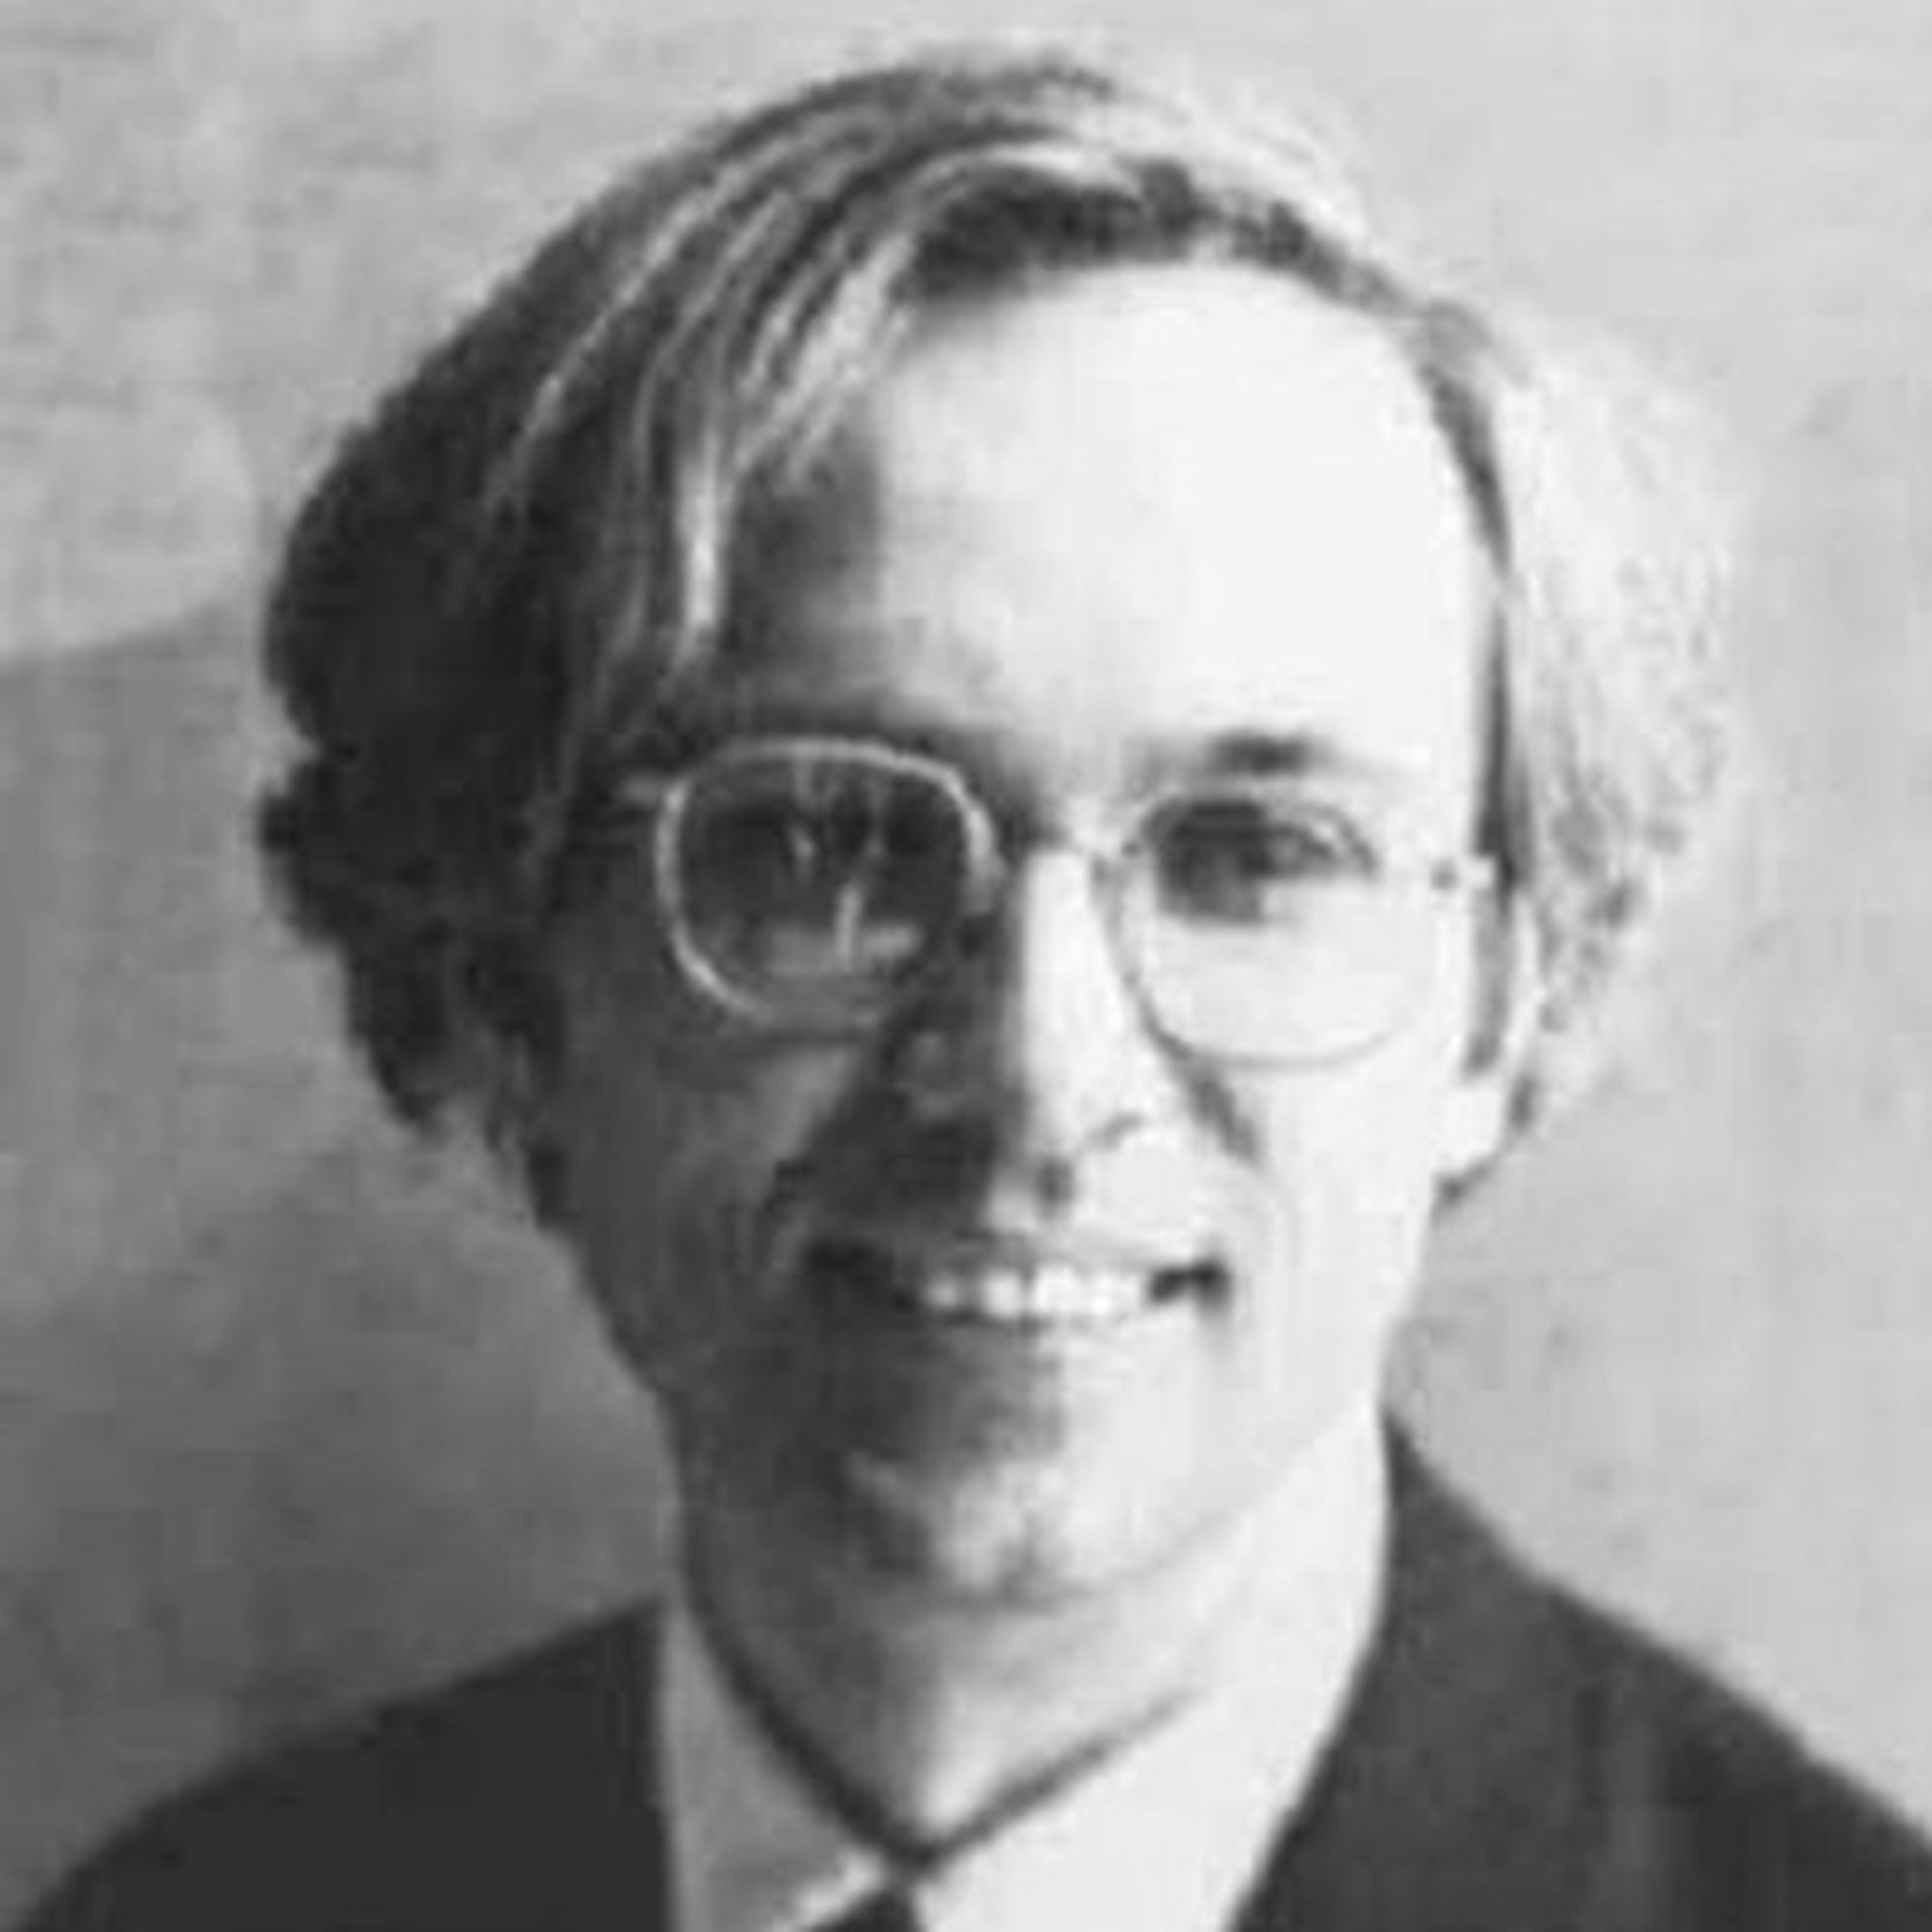
\includegraphics[width=.6\textwidth]{DANIELQ.jpeg}
    
    \label{fig:my_label}
\end{figure}

{\centering \textbf {Daniel Quillen}\par}
\vspace{5mm}
{\centering 1940-2011\par}
\vspace{20mm}

Fue un matemático estadounidense. Es conocido por ser uno de los "primeros arquitectos" de la K-teoría algebraica haciéndolo ganador de la medalla Fields en el 1978. Estudió en la Universidad de Harvard donde se licenció, 1961, y donde obtuvo su PhD. Ha sido profesor en diversas universidades, destacando su estancia en Oxford entre 1984 y 2006, año el que se retiró.
\vspace{5mm}

Inspirado en el matemático Grothendieck La contribución más conocida de Quillen fue su formulación de la teoría K algebraica superior en 1972 donde resolvió el problema K- grupos, $K_n$ para n $\geq$ 3. Esta nueva herramienta, formulada en términos de la teoría de la homotopía, demostró ser exitosa en la formulación y resolución de problemas en álgebra, particularmente en la teoría de anillos y la teoría de módulos. De manera más general, Quillen desarrolló herramientas (especialmente su teoría de categorías de modelos) que permitieron aplicar herramientas algebro-topológicas en otros contextos.




\end{document}